\documentclass{esannV2}
\usepackage[dvips]{graphicx}
\usepackage[latin1]{inputenc}
\usepackage{float}
\usepackage{subcaption}
\usepackage{amssymb,amsmath,array}
\graphicspath{{images/}}

%***********************************************************************
% !!!! IMPORTANT NOTICE ON TEXT MARGINS !!!!!
%***********************************************************************
%
% Please avoid using DVI2PDF or PS2PDF converters: some undesired
% shifting/scaling may occur when using these programs
% It is strongly recommended to use the DVIPS converters, and to submit
% PS file. You may submit a PDF file if and only if you use ADOBE ACROBAT
% to convert your PS file to PDF.
%
% Check that you have set the paper size to A4 (and NOT to letter) in your
% dvi2ps converter, in Adobe Acrobat if you use it, and in any printer driver
% that you could use.  You also have to disable the 'scale to fit paper' option
% of your printer driver.
%
% In any case, please check carefully that the final size of the top and
% bottom margins is 5.2 cm and of the left and right margins is 4.4 cm.
% It is your responsibility to verify this important requirement.  If these margin requirements and not fulfilled at the end of your file generation process, please use the following commands to correct them.  Otherwise, please do not modify these commands.
%
\voffset 0 cm \hoffset 0 cm \addtolength{\textwidth}{0cm}
\addtolength{\textheight}{0cm}\addtolength{\leftmargin}{0cm}

%***********************************************************************
% !!!! USE OF THE esannV2 LaTeX STYLE FILE !!!!!
%***********************************************************************
%
% Some commands are inserted in the following .tex example file.  Therefore to
% set up your ESANN submission, please use this file and modify it to insert
% your text, rather than staring from a blank .tex file.  In this way, you will
% have the commands inserted in the right place.

\begin{document}
%style file for ESANN manuscripts
\title{Sequence learning and recall in recurrent neural networks with time filtered units.}

%***********************************************************************
% AUTHORS INFORMATION AREA
%***********************************************************************
\author{Ram\'on H. Mart\'inez-Mayorquin $^1$, Anders Lansner and $^1$ Pawel Herman $^1$
%
% Optional short acknowledgment: remove next line if non-needed
% \thanks{This is an optional funding source acknowledgement.}
%
% DO NOT MODIFY THE FOLLOWING '\vspace' ARGUMENT
\vspace{.3cm}\\
%
% Addresses and institutions (remove "1- " in case of a single institution)
1- KTH Royal Institute of Technology \\
Department of Computational Science and Technology - Stockholm, Sweden.
%
% Remove the next three lines in case of a single institution
\vspace{.1cm}\\ 
}

%***********************************************************************
% END OF AUTHORS INFORMATION AREA
%***********************************************************************

\maketitle

\begin{abstract}
We demonstrate among others how the learned sequences can be recalled at different speeds largely independent of the encoding process. diojafoids sf dsfsd siofjsdoif
sifjsodif sdjfiosdjf sdio jsdoi fjsoijgi jsoifd jdoifg jodifj iodfj odifjg idfjg
fdjgidfjg djf oidfjgiodfj jdf idfjg odfijg difjg odifjg difg jj dijdfgoidf 
jdfiogjdiofgj 
\end{abstract}

\section{Introduction}
There is a growing interest in studying the capability to learn, store and flexibly recall sequential patterns in neural network models. Processing sequential information bears particular relevance to a wide scope of cognitive functionality and behavior in humans \cite{lashley1951problem}. Hebb proposed that sequential activation of neural cell assemblies, referred to as phases sequences, form the basis of the human thought process \cite{hebb2005organization}. Serial order can be attributed to speech perception and generation, motor control and planning as well as goal directed behavior orchestrated by working memory. Therefore the question as to how a novel sequence of items is stored and recalled in the corrected order has been extensively studied in the context of memory systems among others. Besides intensive efforts in this direction undertaken in the domain of cognitive neuroscience and psychology \cite{hurlstone2014memory} the problem of sequence learning has also attracted a lot of theoretical interest. It has resulted in the development of different computational network models simulating the brain's capabilities to process sequence information. A prominent share of this computaitonal endevaour is linked to spiking neural network approaches to learn precise patterns of spike sequences with biologically plausible local learning rules \cite{ans1994neural}\cite{dehaene1987neural}\cite{gutig2006tempotron}\cite{ponulak2010supervised}. Another group of network approaches developed in the realm of rate based models offers a more generic context for sequence memory function \cite{amari1972learning}\cite{kohonen1977principle}\cite{sandberg2002bayesian}. The work presented here belongs to that category of studies and conceptually builds on \cite{sandberg2002bayesian}. In particular we rely on a simple recurrent neural network architecture and incorporate the concept of synaptic filtering into a basic Hebbian learning rule with synaptic gating \cite{andrew2003spiking} to study the network's capabilities to learn and recall sequences of memory items. The proposed rate based model constitutes a well-controlled framework for studying the fundamental synaptic mechanisms and identifying key parameters responsible for sequence processing capabilities in a dynamical connectionist system with all-to-all recurrent connectivity pattern. 


\section{Methods}

The recurrent neural network in Fig. \ref{Fig:diagrams} is composed of firing rate units with the input-output characteristics described by the logistic function $\Phi(x) = \frac{1}{1 + \exp(-Gx)}$ with gain G. The synaptic inputs are aggregated across the entire network through all-to-all connections weighted by synaptic weights $W$, and the activation of unit $U_i$, is then consistently determined by integrating synaptic inputs with the time constant $\tau_{m}$ (\ref{eq1}). To account for the temporal effect of synaptic smoothing we introduce the idea of z-filters  \cite{tully2016spike} that maintain the exponentially decaying traces of the activity with the time constant of $\tau_z$ (\ref{eq2}). This allows for keeping synaptic memory of the unit activity and influencing other post-synaptic units in the network even when the original pre-synaptic unit is not longer active. 

\begin{align}
\tau_m \dfrac{dx_i}{dt} &= \Phi\Big(\sum_{j} W_{ij} z_j - \theta \Big) - x_i \label{eq1} \\ 
\tau_z \dfrac{dz_i}{dt} &= x_i - z_i \label{eq2}
\end{align}



In this work we examine two types of learning rules, pre-synaptic (3) and post-synaptic (4)
gating \cite{andrew2003spiking}, which equip the proposed network with the capability to learn
how to recall sequential activity patterns.

\begin{align}
\tag{3 pre-synaptic}
\tau_w \dfrac{dw}{dt} &= (w_{max} - w) z_{pre}z_{post} + (w_{min} - w) (1 - z_{post})z_{pre} \label{eq:pre-synaptic rule}  \\
\tag{4 post-synaptic}
\tau_w \dfrac{dw}{dt} &= \underbrace{(w_{max} - w)}_{\text{saturation}} \underbrace{z_{pre}z_{post}}_{\text{Hebbian}} + \underbrace{(w_{min} - w)}_{\text{saturation}}\underbrace{ (1 - z_{pre})z_{post}}_{\text{synaptic-gating}} \label{eq:post-synaptic rule}
\end{align}

\begin{figure}[H]
\centering
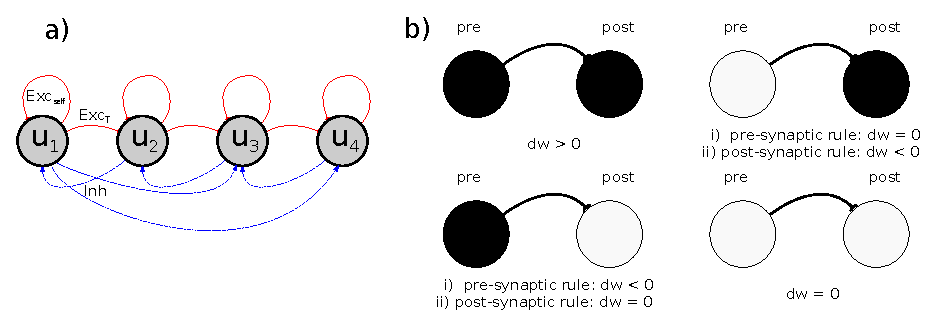
\includegraphics[scale=0.8]{diagram_mixed.eps}
\caption{a) Scheme of the overall network connectivity of the system. Note that the inhibitory connections are only fully depicted for the first unit for the sake of clarity. b) Conceptual illustration of the mechanism of learning induced synaptic changes. Here the a black filling stands for an active unit. } \label{Fig:diagrams}
\end{figure}


The first term in (\ref{eq:pre-synaptic rule}) and (\ref{eq:post-synaptic rule}) is an associative Hebbian contribution \cite{hebb2005organization} and its role is to strengthen the connections between activated units. Importantly however, in comparison with the original formulation \cite{andrew2003spiking}, we use the z-filters instead of the unit activities. This provides the scope for making associative connections between units even when either of the two units is no longer active provided that its memory trace is retainedby the synapse. As mentioned earlier, the synaptic trace decays exponentially with the time constant of $\tau_z$ (\ref{eq2}), and to preserve serial recall order we introduce asymmetrical time constants for z-pre and z-post : $\tau_{z_{pre}} > \tau_{z_{post}}$. The second term is called synaptic gating \cite{andrew2003spiking}, which facilitates the formation of inhibitory connections whenever the activity (or its z-filtered trace) of one unit is not accompanied with the activity of the other unit. We examine two variations of this term to explore the functional implications of both pre- and post-synaptic gating. Finally, the weights are kept between $w_{min}$ and $w_{max}$ limits. The nature of synaptic changes under the synaptic gating rule is illustrated in Fig. \ref{Fig:diagrams}.

%\begin{figure}[h!]
%\centering
%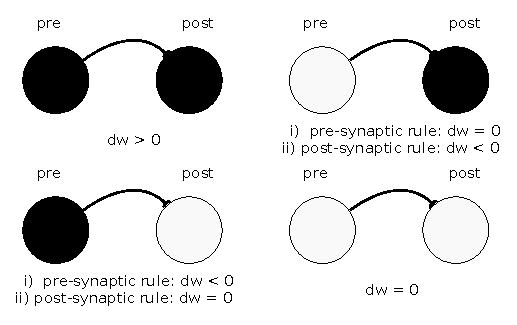
\includegraphics[scale=1.3]{plasticity_diagram.eps}
%\caption{Conceptual illustration of the mechanism of learning induced synaptic changes. Here the a black filling stands for an active unit a) Hebbian associative plasticity that implies a weight increase when both pre- and pos-synaptic units are simultaneously active b) In the case of the post-synaptic rule the weight is decreased if the post-synaptic unit itself active without the pre-synaptic unit being active. c) In the case of the pre-synaptic rule the weight is decreased if the pre-synaptic unit is itself active without the post-synaptic unit being active. d) If neither pre- nor post-synaptic units are active, there is no weight modification.}\label{Fig:plasticity diagram}
%\end{figure}
%
As a result of learning described above, three types of connections emerge from each unit (Fig. \ref{Fig:diagrams}): two excitatory connections - self-reinforcing unit activity, $Exc_{self}$, and exciting the following unit in the sequence (contributing to the sequential structure of the activity) $Exc_T$, and a range of inhibitory connections, $Inh$, to all the remaining units (among inhibitory connections of special relevance are the backwards inhibitory projections that suppress the unit activity once the next unit in the sequence gets activated).


\section{Results}

\subsection{The neural network can sustain sequential activity}

To recall a particular sequence we cue the first sequence item (unit) by injecting a short input lasting around $\tau_z$. After this initial cue, if the weights have the right configuration as a result of training, the neural network continues to visit subsequent items in the learned sequence to the very
end, as shown in Fig. \ref{Fig:recall}. 


\begin{figure}[h!]
\centering
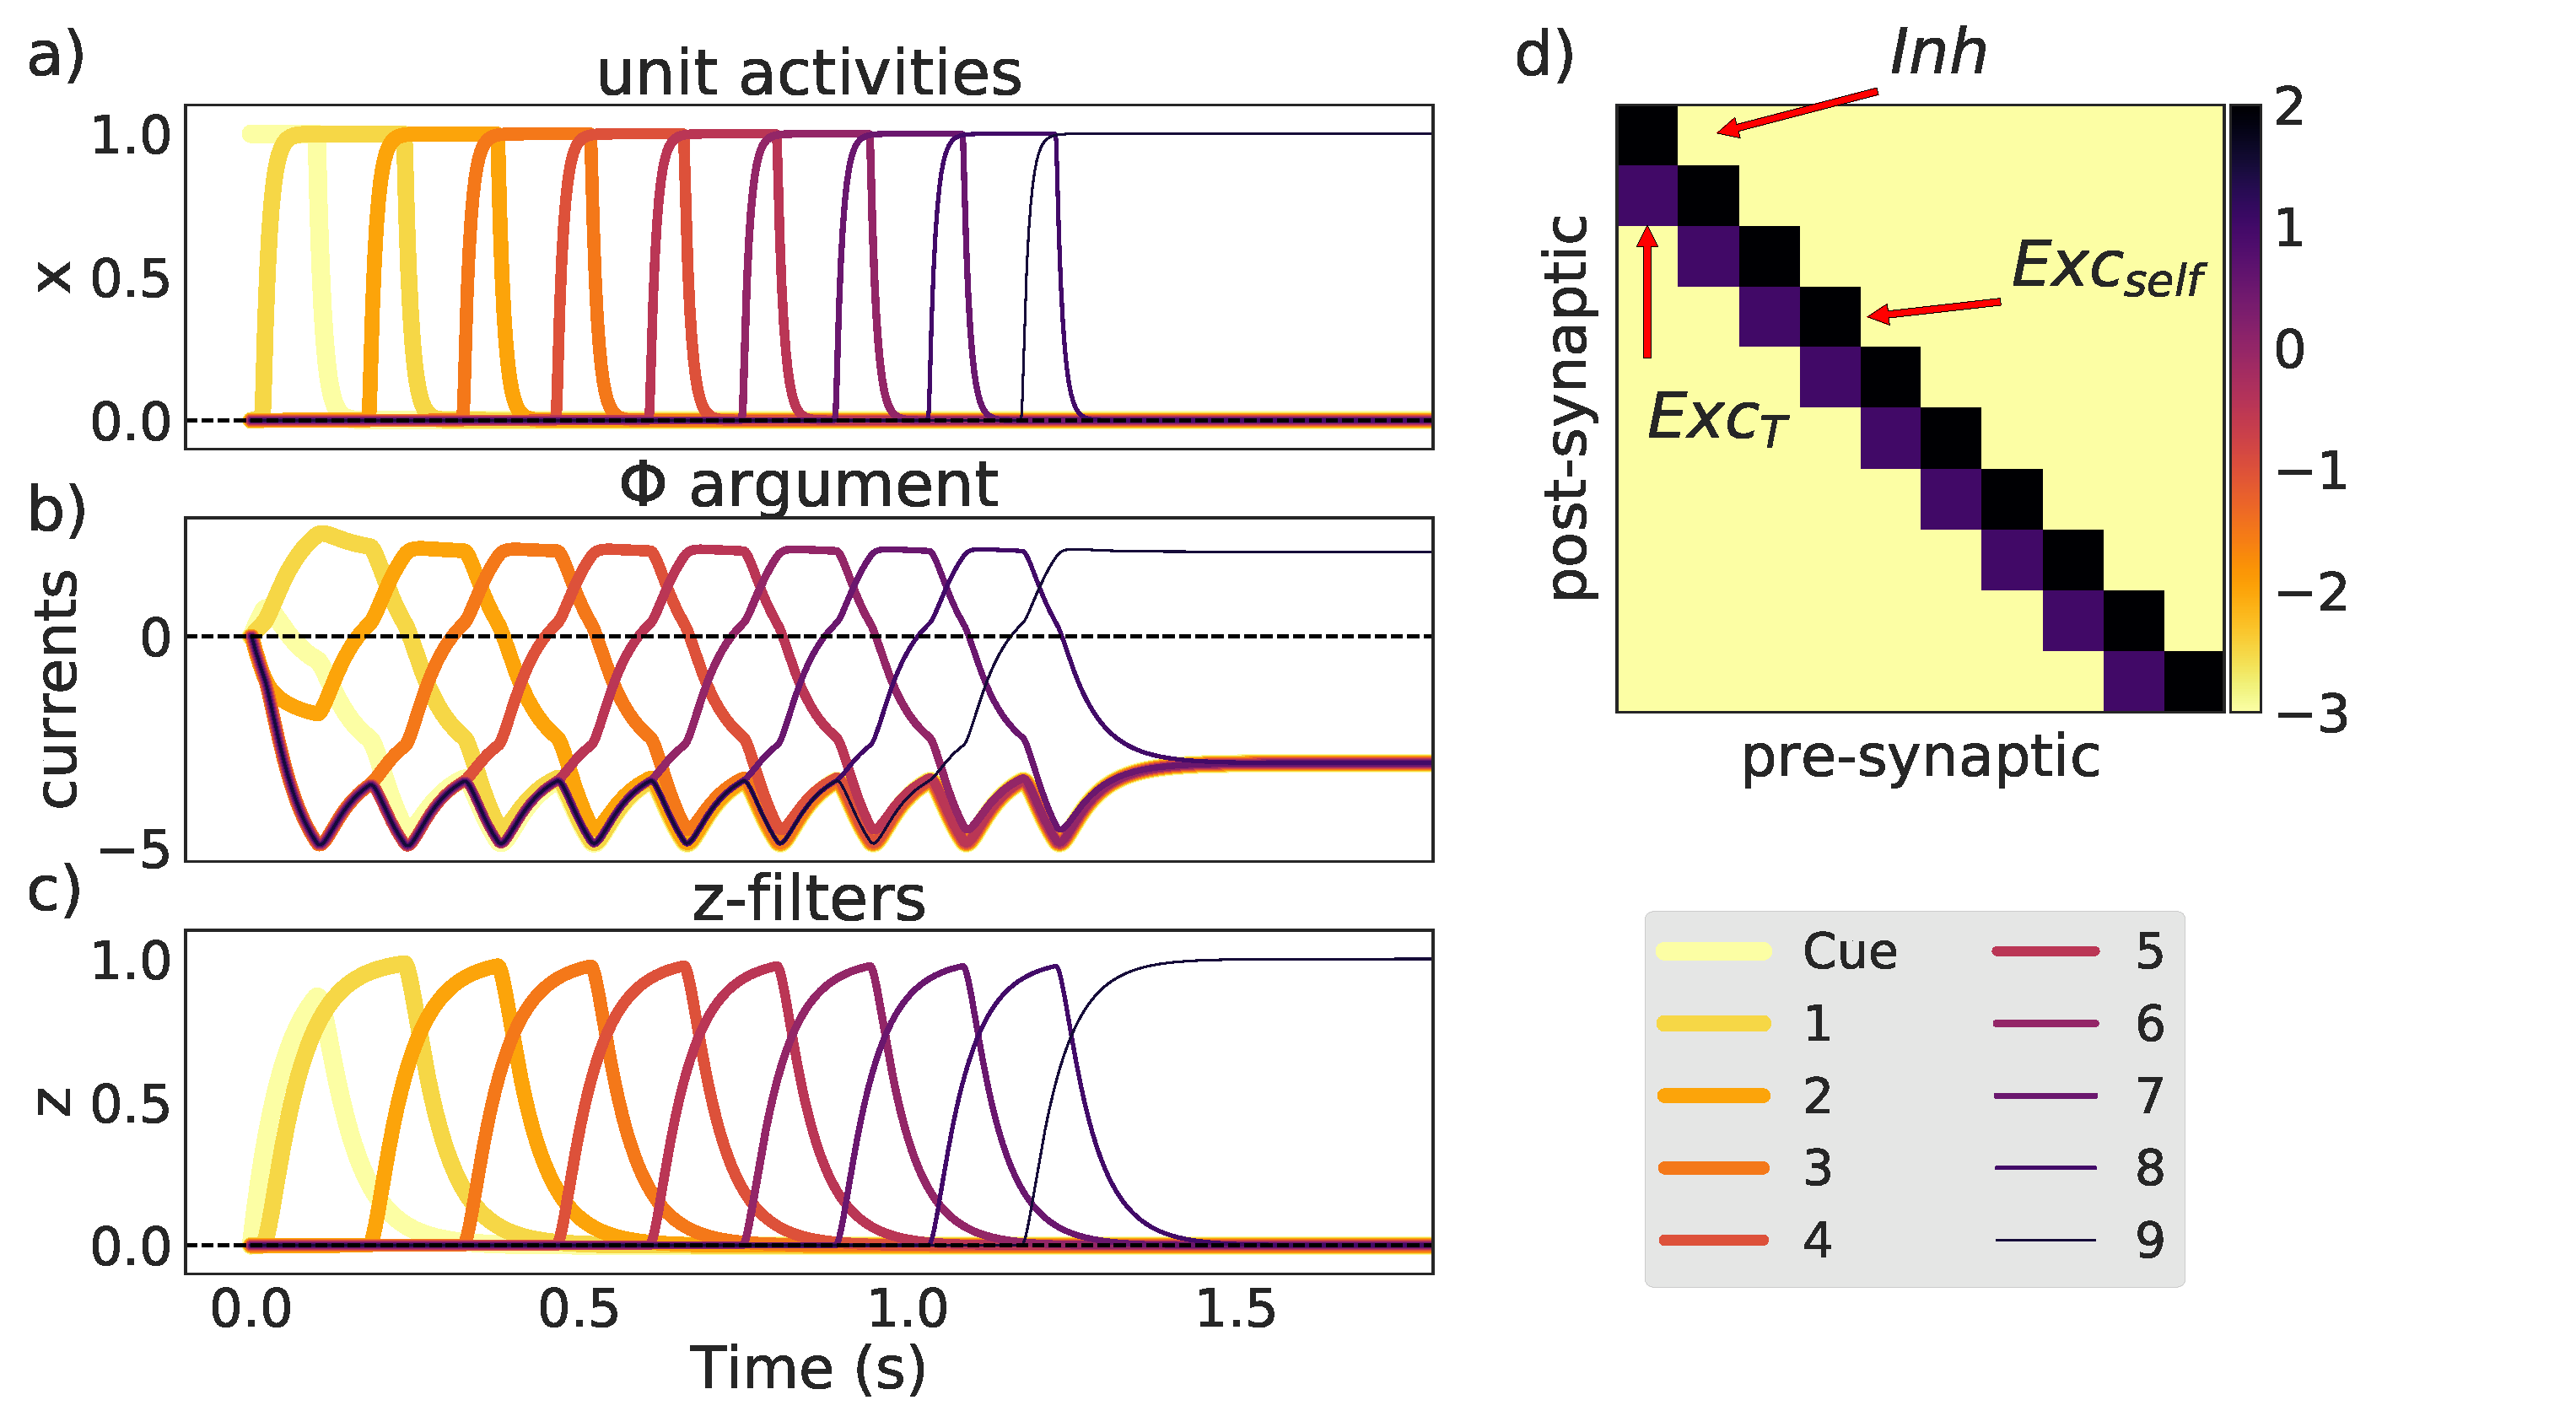
\includegraphics[scale=0.20]{recall.eps}
\caption{Demostration of the successful sequence recall with the corresponding connectivity matrix. a) The activity of the units over time. b) The currents that each unit receives as the sequence progresses. c) the z-filters activations for each unit. d) The connectivity matrix $W$. The weights of the matrix $W$ can be divided into the excitatory connections: the ones on the diagonal that stabilize the unit $Exc_{self}$, the ones under the diagonal that induce transitions $Exc_{T}$ and finally the ones that stabilize the unit  and the inhibitory connections $Inh$ which dominate the matrix $W$. We use different colors to represent different items. }\label{Fig:recall}
\end{figure}


The dynamics of the sequential activity propagation can be easily explained. After the first unit $U_1$ has been activated by the external input, the corresponding filter $z_1$ starts following the activity $x_i$. In consequence, the subsequent unit $U_2$ receives a growing current with value $z_1 Exc_T$ because of the forward connectivity. This process continues until the point in time when $Exc_{T}(1 - e^{-\frac{t}{\tau_z}}) - \theta = 0$ implying that $U_2$ receives enough current to become activated. This in turn prompts the filter $z_2$ to follow the activity $x_2$ initializing again the process described above. On the other hand as soon as the synaptic trace corresponding to $x_2$ starts growing, the preceding unit $U_1$ beings to receive an inhibitory current $z_2 Inh$ due to the backward inhibitory projection. This in turn suppresses the activity of unit $U_1$ facilitating the propagation of the sequence. Finally once the unit $U_1$ is completely suppressed the excitatory current mediated by $Exc_T$ is diminished, which in most cases would also suppress the activity $x_2$ if it was not for the self-sustaining current $z_2 Exc_{self}$. In short, the term $Exc_T$ ensures the transition of the activity from one network state (sequence item) to another one (the next item in the sequence) whereas the competition between $Exc_{self}$ ad $Inh$ first lock the pattern unit and then finally suppresses it enabling the sequence to continue its trajectory. 


With the knowledge above in mind we can envision the following  failure scenarios for the sequential dynamics. First, if the magnitude of $Exc_{self}$ weight is small the self-excitatory current is not sufficiently strong to overcome the threshold and the sequence stalls. Second, if $Exc_{self}$ is large enough to keep the unit active but the $Exc_{T}$ weight is weak, the next unit in the sequence does not become activated and the sequence remains stuck forever in the same state corresponding to the first pattern. Finally if both $Exc_{self}$ and $Exc_T$ are strong enough to sustain and propagate the activity respectively but the inhibitory weight $Inh$ is not sufficiently large to suppress the activity, all the units in the sequence become co-activated at the end. 

\subsection{The neural network possess a wide dynamic range}

A common problem in sequence learning is to scale the time duration of the sequence according to the contextual demands \cite{murray2017learning}. For a neural network it means that the dynamics of sequence recall can be flexibly controlled with the network parameters after the training process is completed. The recall time can be defined as the temporal length of the activation of the individual units during the sequence retrieval. In the network there are two key parameters that are directly implicated in the regulation of the recall time: the transition weight, $Exc_T$ and the threshold, $\theta$, which control how long it takes to recruit the next unit in a sequence. Below we derive the estimate of how $Exc_T$ affects the recall time and the reasoning for $\theta$ is analogous. 



In order to calculate the recall time we make the following consideration. Once the unit $U_1$ becomes activated the filter $z_1$ starts growing thereby contribution to the excitatory current input, $z_1 Exc_T$, to the next unit $U_2$. The point in time at which this current overcomes the threshold marks the end of the recall process for a specific item in the sequence. Following that reasoning we can solve the equation $Exc_{T}(1 - e^{-\frac{t}{\tau_z}}) - \theta = 0$ to estimate the recall time. As a result, we obtain the following expression:

\begin{align}
T_{recall} = \tau_z \log\Big(\frac{Exc_T}{Exc_T - \theta} \Big)
\end{align}

This expression has a singularity at $Exc_T = \theta$, which implies that the recall time can be made arbitrarily long by setting $Exc_T$ close to the threshold. However due to the all-to-all connectivity the are other contributions which we can take into account with:

\begin{align}
T_{recall} = \tau_z \log\Big(\frac{Exc_T + Inh}{Exc_T - \theta}\Big) \label{eq:recall_complex}
\end{align}

Figure \ref{Fig:dynamical_range} illustrates the wide dynamical range of the recall time in our network model (both simulated and estimated as presented above)


\begin{figure}[h!]
\centering
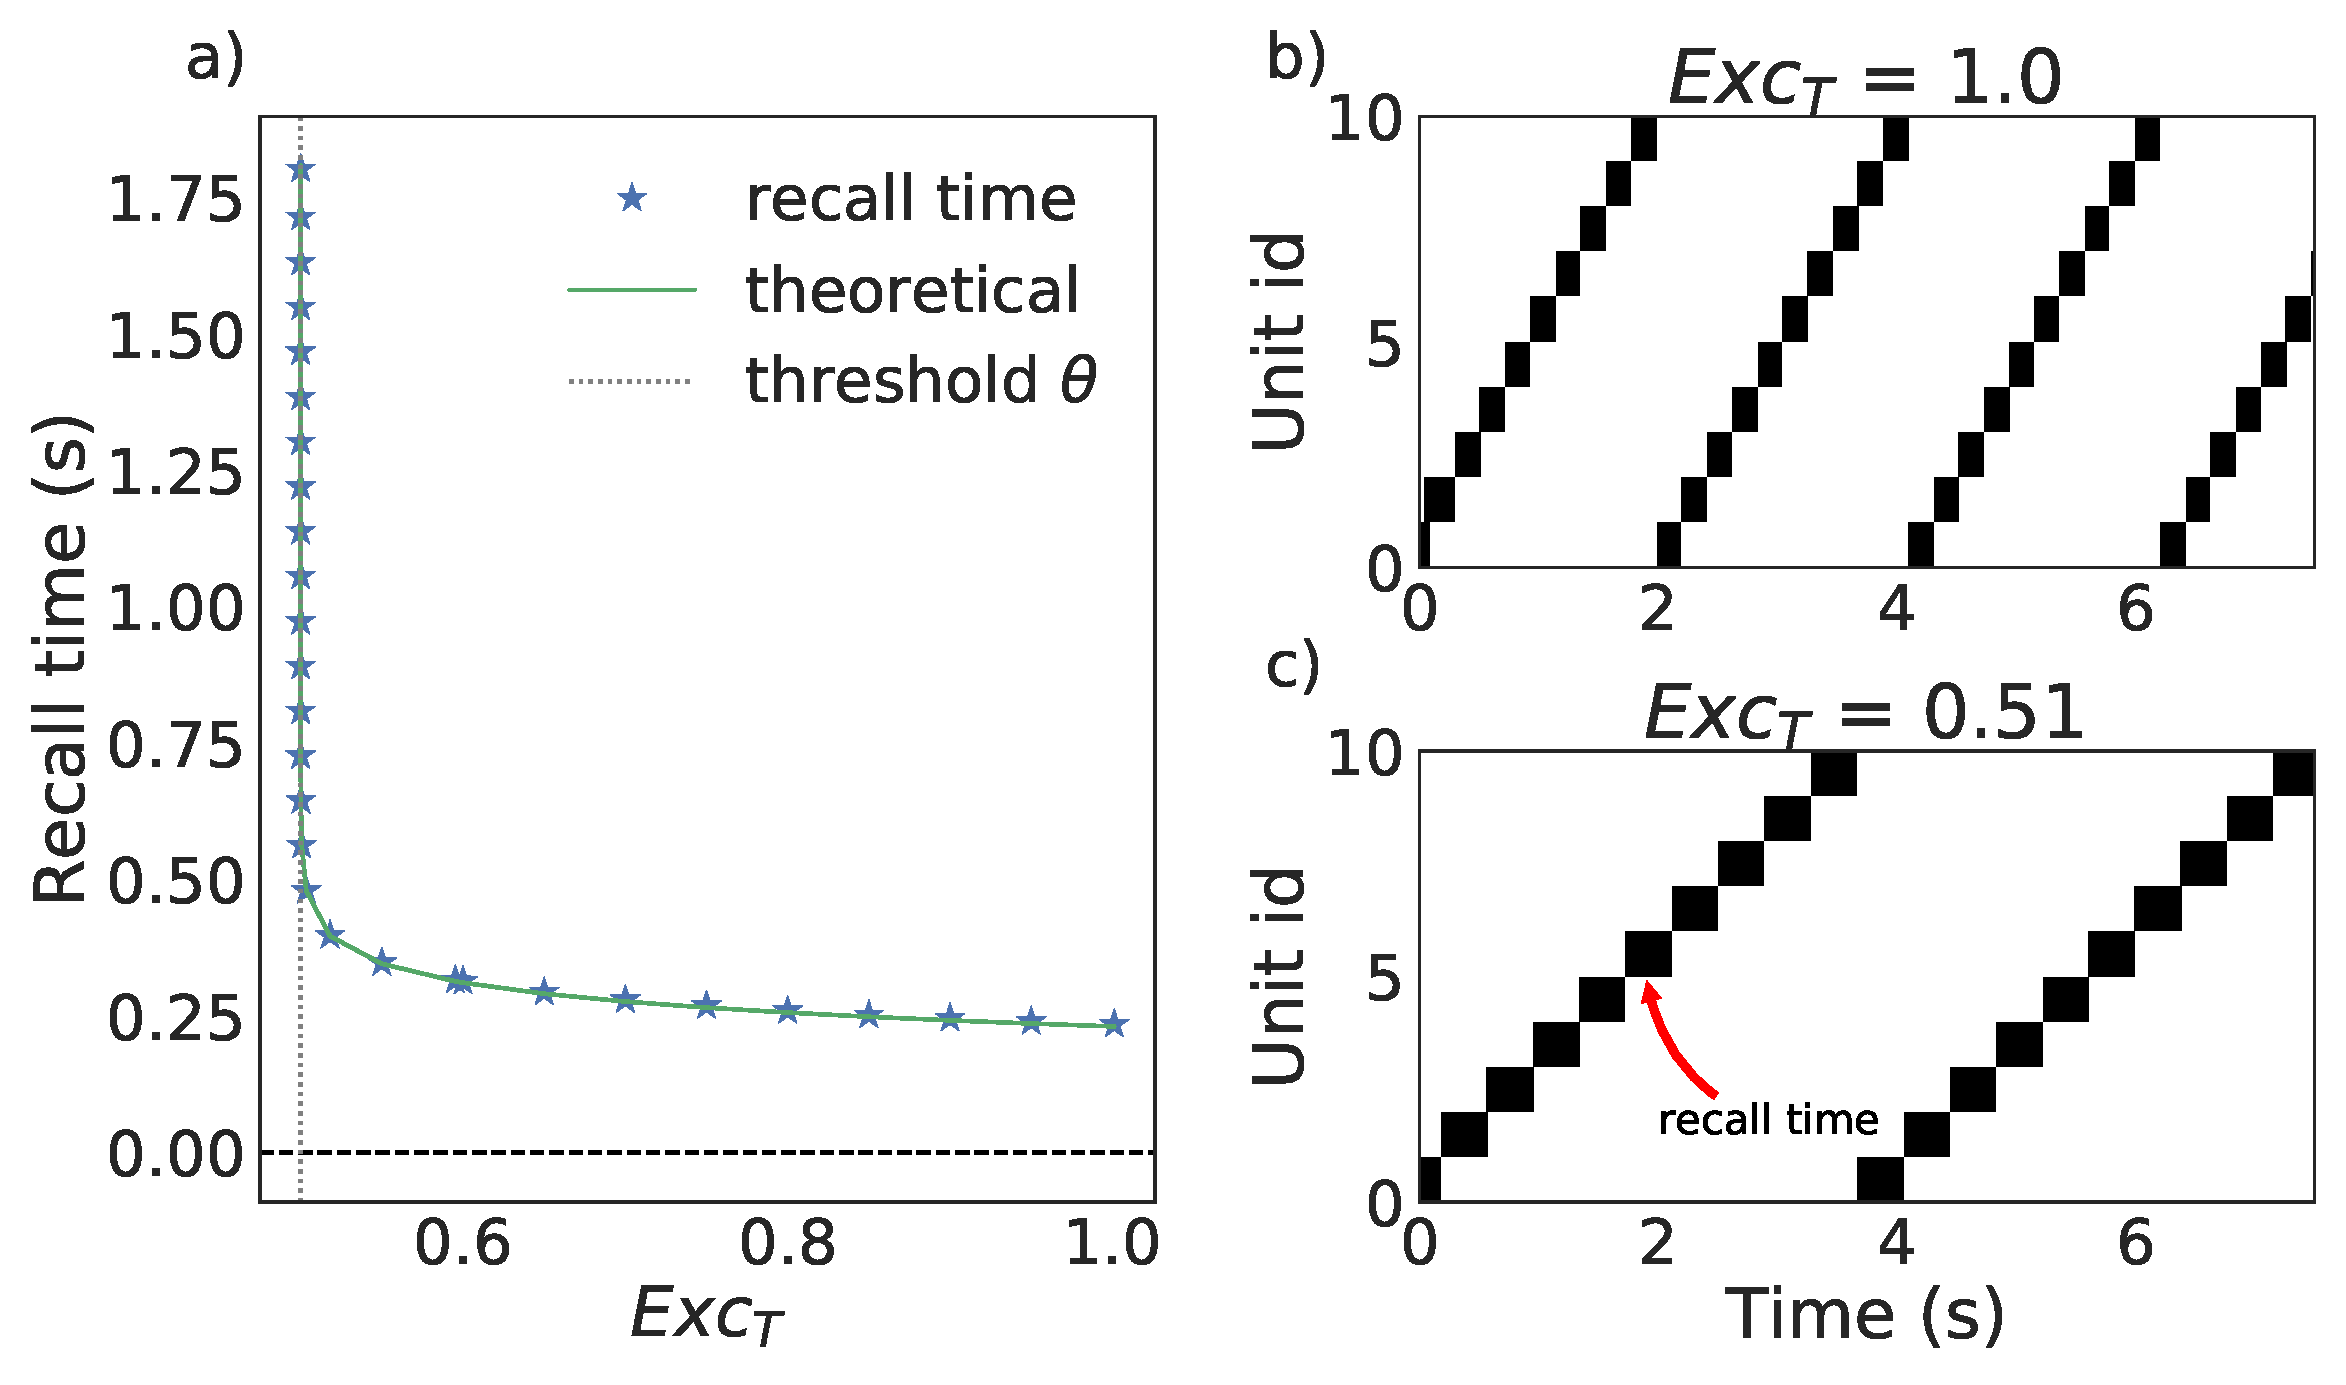
\includegraphics[scale=0.28]{dynamical_range.eps}
\caption{The network posses a wide dynamical range. a) Here we compare the calculated thoretical expression with simulations with our network for different values of $Exc_T$. Note the singularity at $\theta$. b) The network activity with a short recall time. c) The network activity with a longer recall time ($Exc_T$ close to $\theta$).}\label{Fig:dynamical_range}
\end{figure}



\subsection{Learning Rule}
Our learning protocol consists in fixing (clamping) each unit of the sequence in succession for a given amount of time (training time). We perform this process an epochs number of times. It is important to note that while learning there is a period of one second between each epoch or presentation that serves the purposes of avoiding self-interference.  


\begin{figure}[H]
\centering
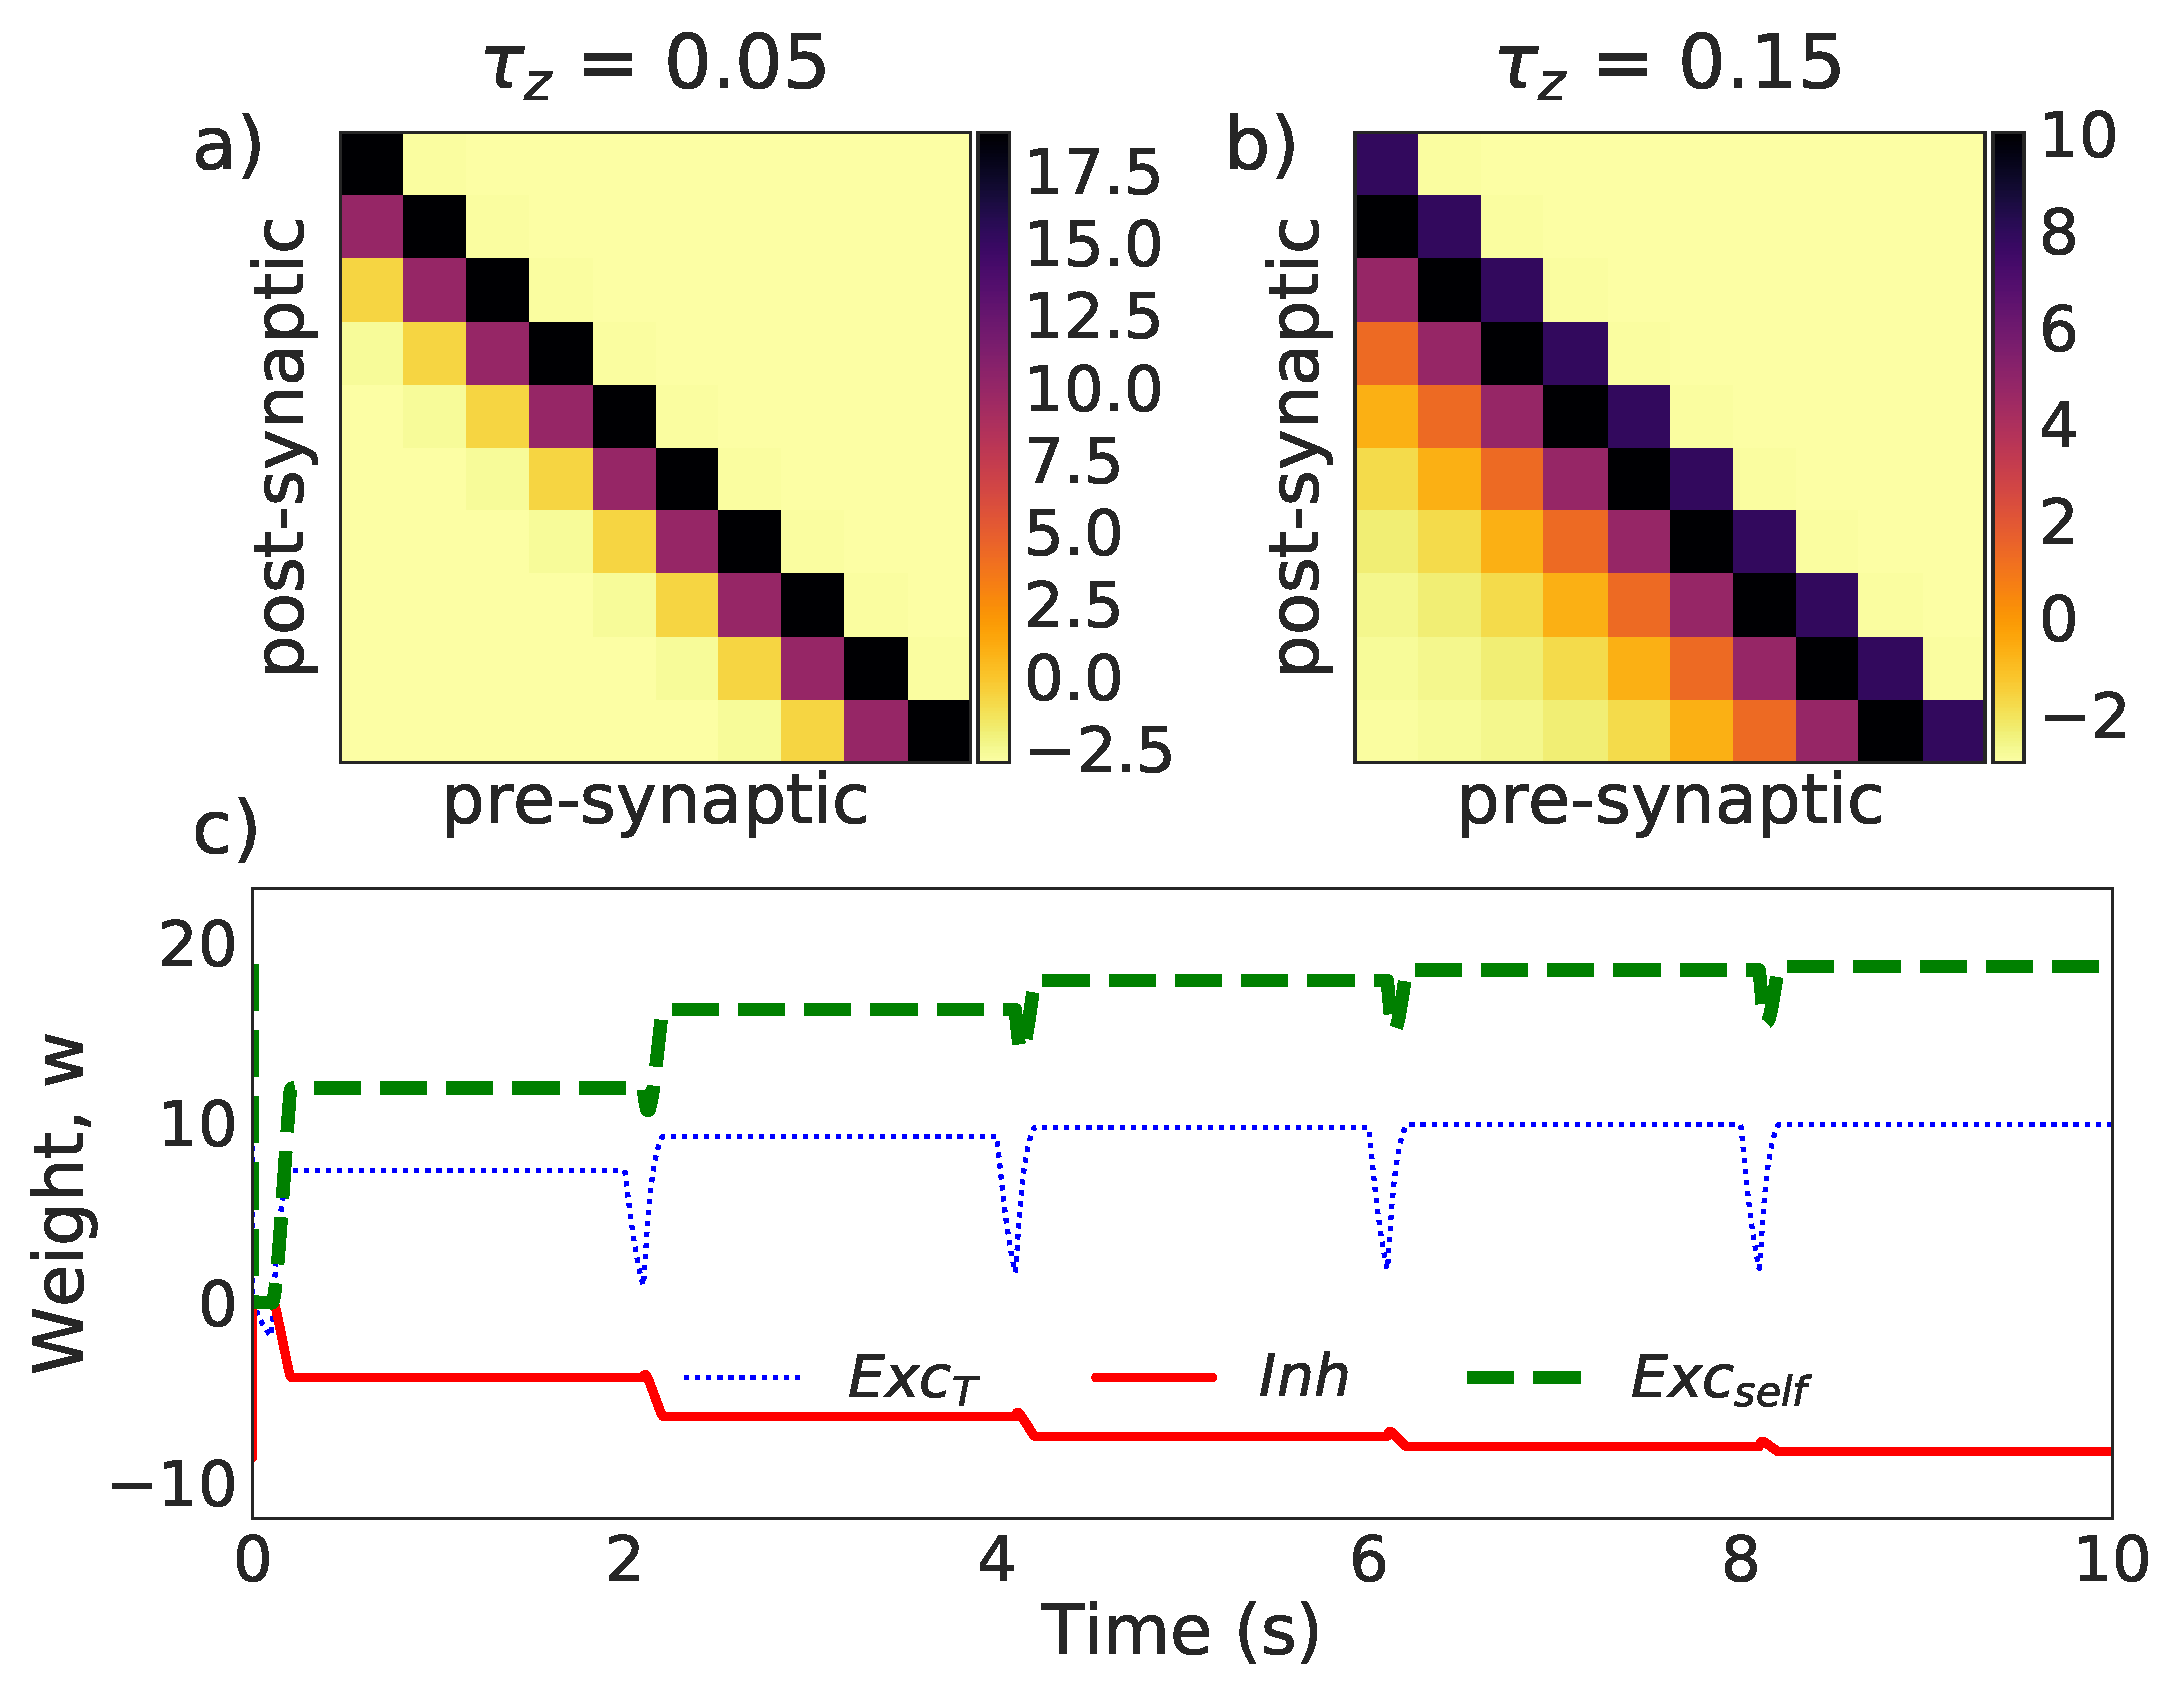
\includegraphics[scale=0.3]{training_rule.eps}
\caption{The effect of training with the learning rule. a) An example of training with a small value of $tau_z=0.050s$. b) Same procedure as in a but with a longer time constant $\tau_z=0.150s$. c) evolution in time of the connection weights from the first to the second unit $Exc_T$, the one from the second back to the first unit $Inh$ and finally of the second unit into itself $Exc_{self}$. Five epochs of length $2s$ are shown here, note that this is enough time for the weights to stabilize.}\label{Fig:epochs}
\end{figure}



%\begin{figure}[H]
%\centering
%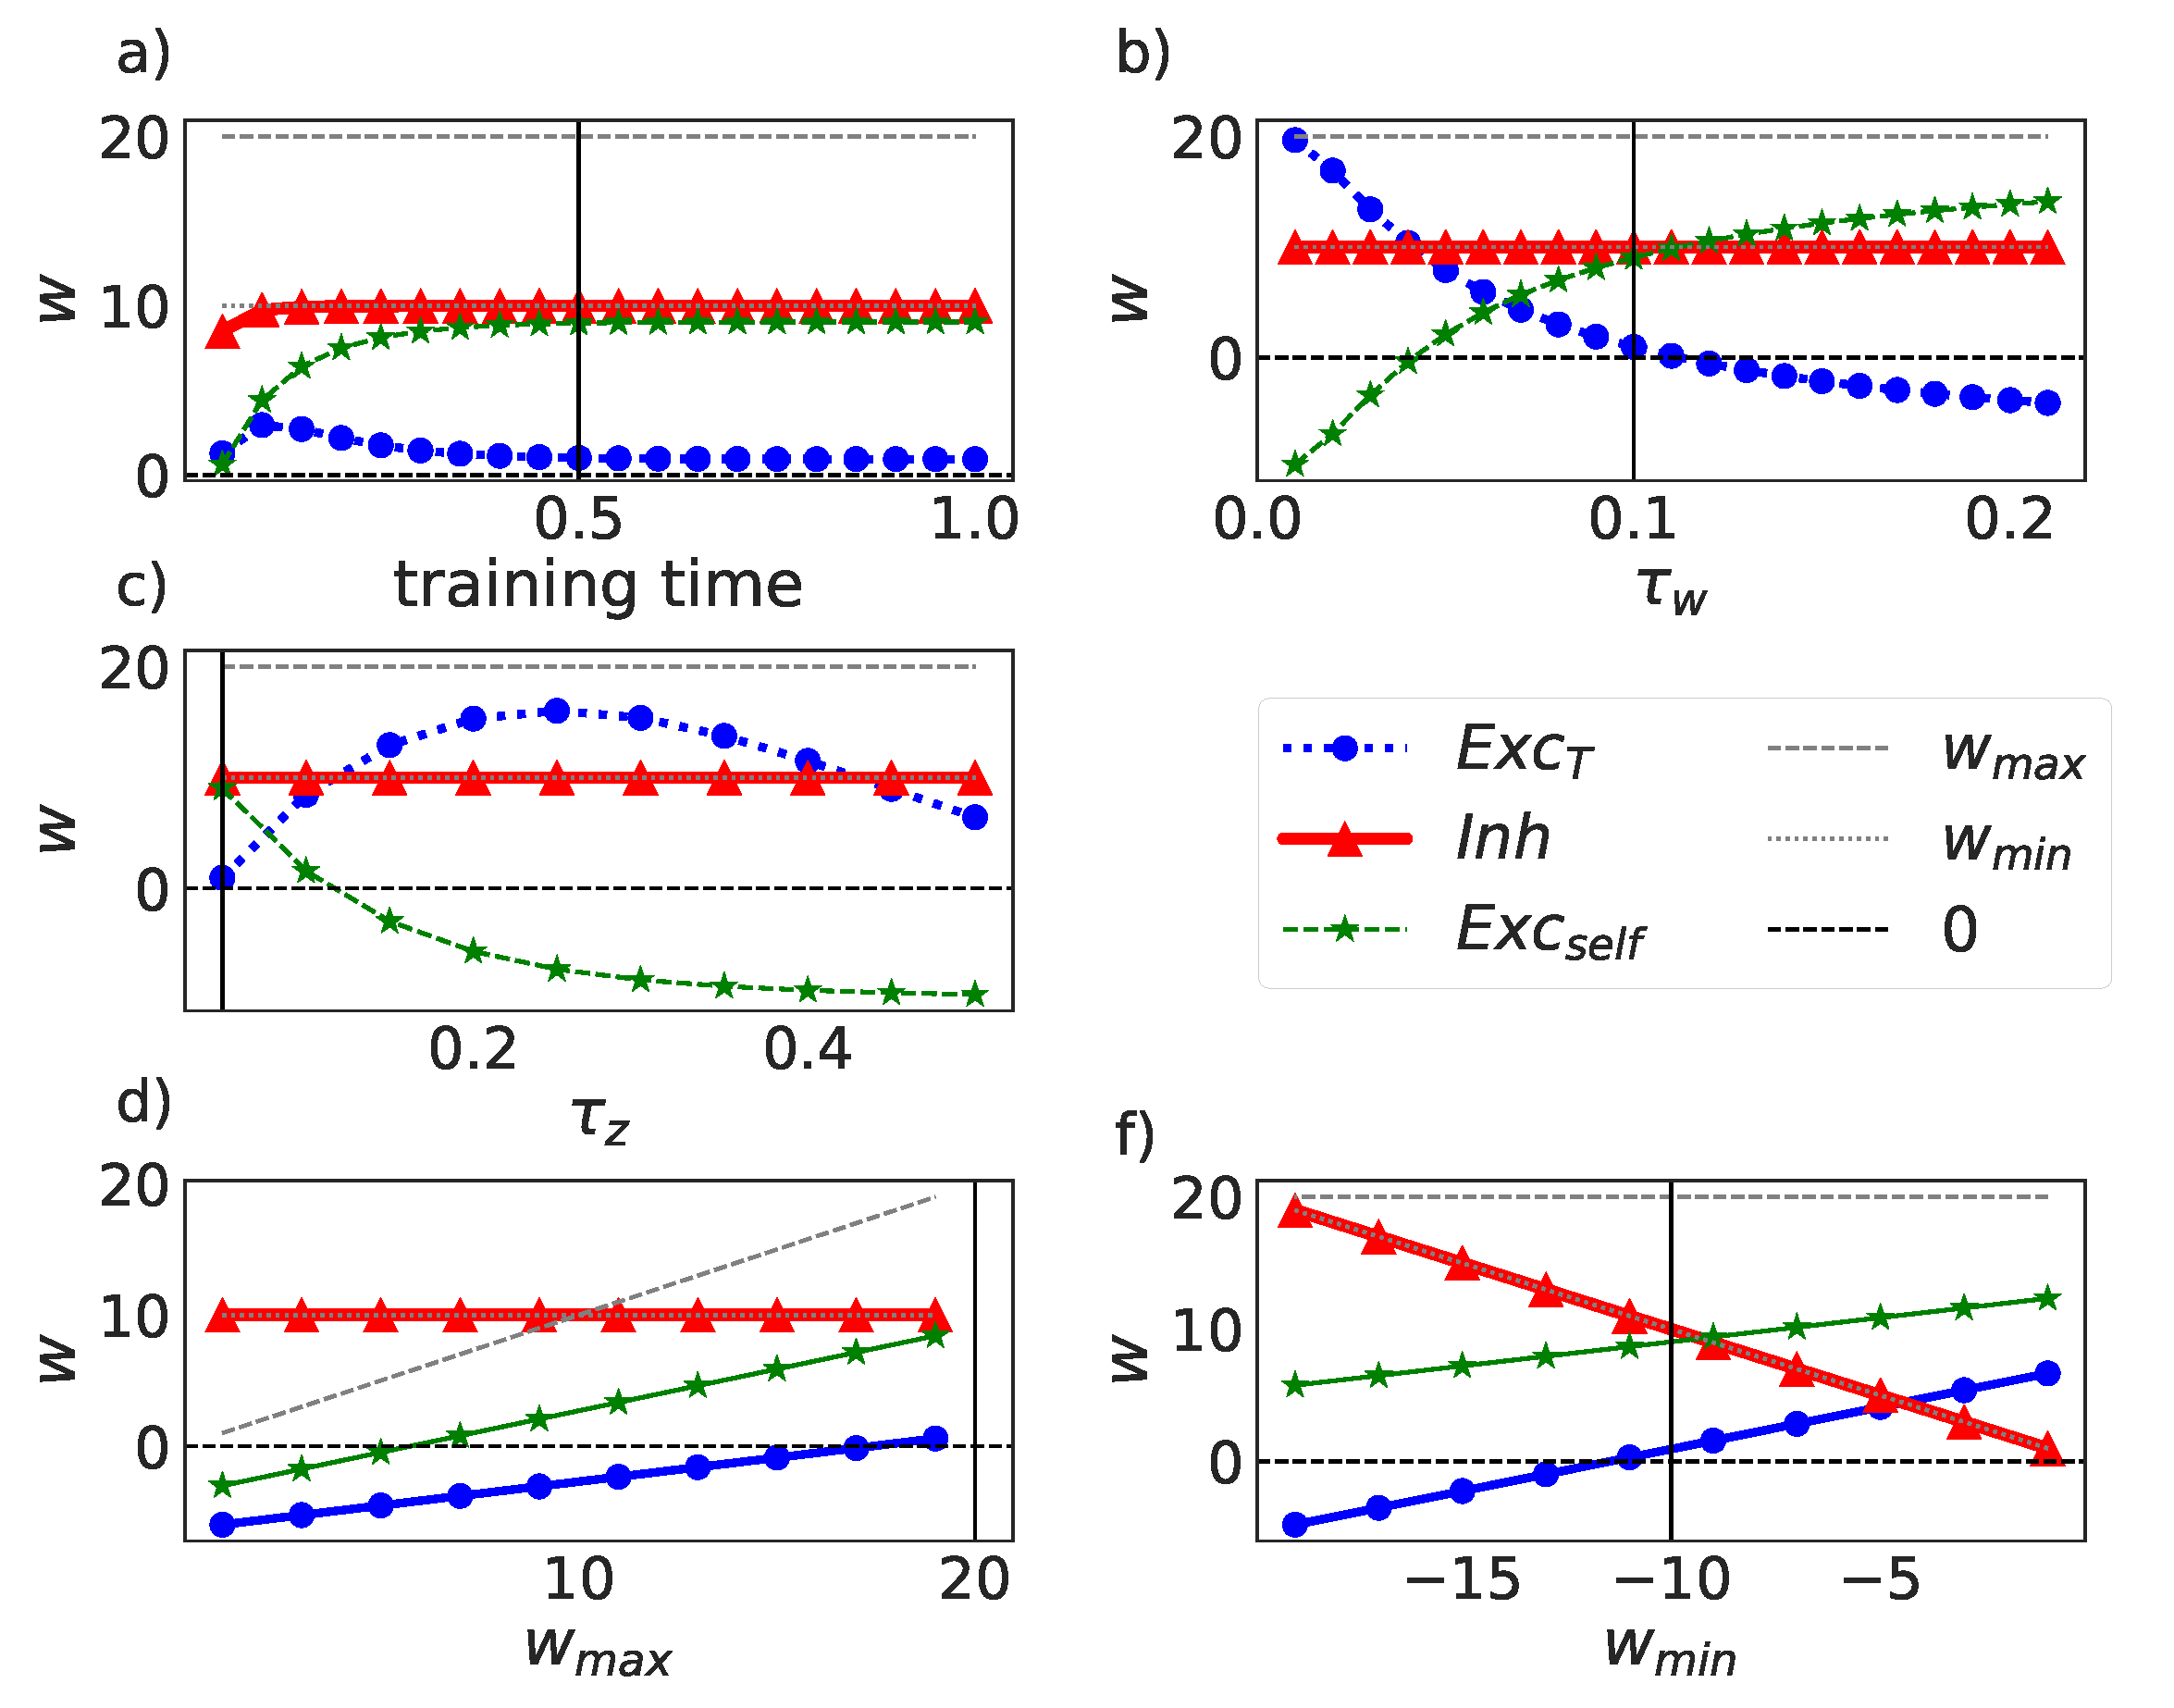
\includegraphics[scale=0.3]{training_rule_quantities_pre_rule_True.eps}
%\caption{Learning dynamics of the pre-synaptic learning rule.}\label{Fig:learning_quantities_pre}
%\end{figure}
%
%
%\textbf{Training time}
%\begin{itemize}
%\item  $Exc_{self}$: The longer the training time the longer the filter is activated with itself and therefore it grows. But given that the pre and post filters do not coincide completely in the temporal domain there are negative contributions which prevent this from reaching the saturation value $w_{max}$
%\item  $Inh$: In this case the the negative contributions come from the time that the units are not activated together with their counterparts which is most of the time (except in the brief transition period) and therefore the value saturates quickly to $w_{min}$.
%\item $Exc_{T}$: In this case what matters is the transition time between two 
%\end{itemize} 
%
%
%\begin{figure}[H]
%\centering
%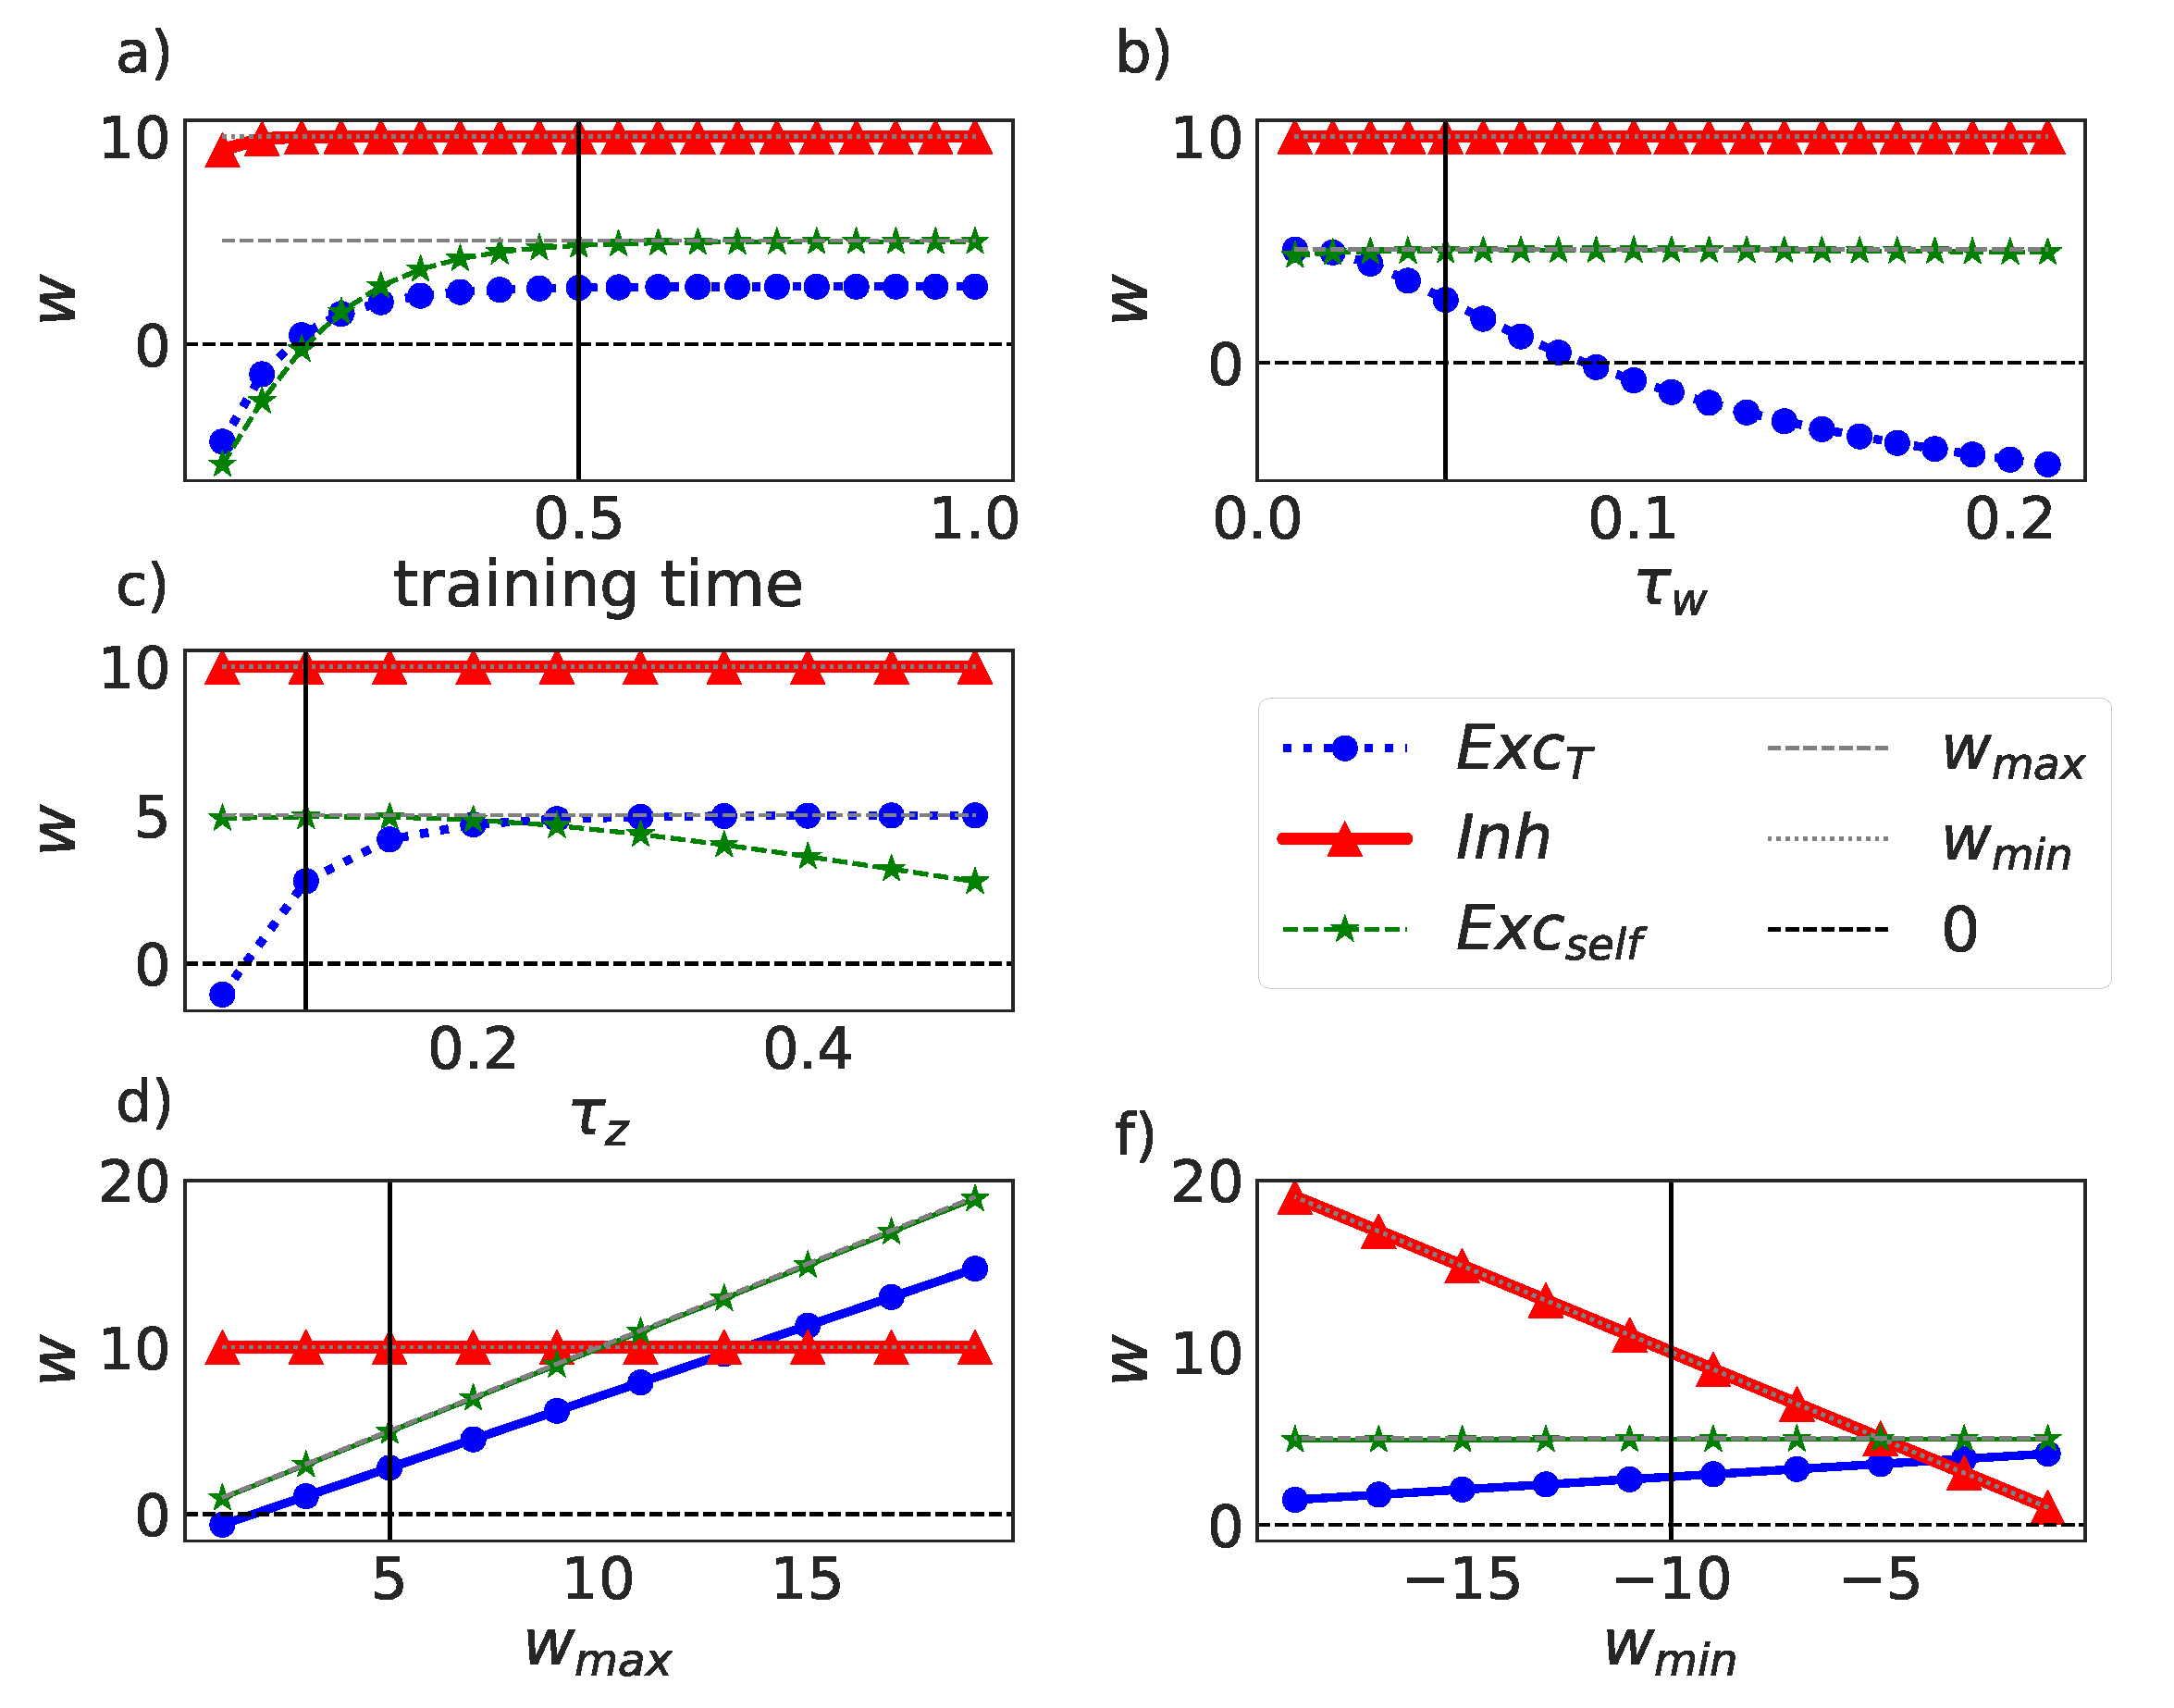
\includegraphics[scale=0.3]{training_rule_quantities_pre_rule_False.eps}
%\caption{Learning dynamics of the post-synaptic learning rule}\label{Fig:learning_quantities_post}
%\end{figure}

 


\section{Discussion}


% ****************************************************************************
% BIBLIOGRAPHY AREA
% ****************************************************************************

\begin{footnotesize}

% IF YOU USE BIBTEX,
% - DELETE THE TEXT BETWEEN THE TWO ABOVE DASHED LINES
% - UNCOMMENT THE NEXT TWO LINES AND REPLACE 'Name_Of_Your_BibFile'

\bibliographystyle{unsrt}
\bibliography{references.bib}

\end{footnotesize}

% ****************************************************************************
% END OF BIBLIOGRAPHY AREA
% ****************************************************************************

\end{document}
